\documentclass[12pt,a4paper]{article}

\usepackage[utf8]{inputenc}
\usepackage[T2A]{fontenc}
\usepackage[english,russian]{babel}

\usepackage{geometry}
\usepackage{float}

\usepackage{gensymb}

\usepackage{amsfonts,amscd}
\usepackage{amssymb,amsmath,amsthm,enumerate}

\usepackage{graphicx}
\usepackage{authblk}
\usepackage{titlesec}
\usepackage{hyperref}
\usepackage{etoolbox}

\usepackage{array}
\usepackage[parfill]{parskip}
\usepackage{caption}
\usepackage{subcaption}
%\captionsetup[figure]{labelformat=empty}

\usepackage{bm}
\usepackage{bbm}

%\usepackage{gensymb}
\usepackage[]{units}
\usepackage{listings}

\usepackage{physics}

\usepackage{xurl}
\usepackage{tabto}

\usepackage{multirow}
\usepackage{multicol}
\usepackage[bottom]{footmisc}
\usepackage{booktabs}

\usepackage[table]{xcolor}
\usepackage[clean]{svg}

\newtheorem{theorem}{Лемма}

\setlength{\parskip}{1em}

\geometry{a4paper,left=20mm,top=30mm,bottom=30mm,right=20mm}

\makeatletter
\patchcmd{\chapter}{\if@openright\cleardoublepage\else\clearpage\fi}{}{}{}
\makeatother % new chapter on the same page
\hypersetup{colorlinks=true, citecolor=blue, linkcolor=blue, urlcolor=blue} % links and clickable ToC
\titleformat{\chapter}
{\normalfont\LARGE\bfseries}{\thechapter}{1em}{}
\titlespacing*{\chapter}{0pt}{3.5ex plus 1ex minus .2ex}{2.3ex plus .2ex} % to redefine some margins
\author{Sergei Makeev}
\title{Poisson equation numerical solution}
\begin{document}
    \begin{titlepage}
        \begin{center}
            
\includegraphics[height=0.9in]{logo.png}\\
            \textsc{\large{\bfseries МОСКОВСКИЙ ГОСУДАРСТВЕННЫЙ УНИВЕРСИТЕТ ИМ. М.В. ЛОМОНОСОВА}} \\	
            \line(1,0){400} \\
            [5mm]
            \textsc{\large{\bfseries ФАКУЛЬТЕТ ВЫЧИСЛИТЕЛЬНОЙ МАТЕМАТИКИ И КИБЕРНЕТИКИ}} \\
            [4cm]
            \textsc{\Large{\bfseries Отчет по заданию по курсу \\
            «Суперкомпьютерное моделирование и технологии»{}}} \\
            [4cm]
        \end{center}
        \begin{flushright}
            \textsc{Сергей Макеев, 617 гр.}
        \end{flushright}
        \vfill
        \begin{center}
            
            \today
        \end{center}	
    \end{titlepage}
    \tableofcontents
    \newpage

    \section{Постановка задачи}

    Необходимо приближённо решить двумерную задачу Дирихле для уравнения Пуассона в криволинейной области. В качестве области $D$ выбран тупоугольный треугольник с вершинами в точках $C(-3, 0)$, $A(3, 0)$, $B(0, 2)$.

    В области $D \subset \mathbb{R}^2$, ограниченной кусочно-гладким контуром $\gamma$, рассматривается дифференциальное уравнение Пуассона:

    $$
    -\Delta u = f(x, y),
    $$

    где $\Delta u = \frac{\partial^2 u}{\partial x^2} + \frac{\partial^2 u}{\partial y^2}$ — оператор Лапласа, а функция $f(x, y)$ считается известной. В данном случае $f(x, y) = 1$ для всех $(x, y) \in D$.

    Для выделения единственного решения уравнение дополняется граничным условием Дирихле:

    $$
    u(x, y) = 0, \quad (x, y) \in \gamma.
    $$

    Задача состоит в нахождении функции $u(x, y)$, которая удовлетворяет уравнению Пуассона в области $D$ и краевому условию на её границе $\gamma$.


    \section{Численный метод решения}

    Для приближённого решения задачи Дирихле для уравнения Пуассона в криволинейной области применяется подход, включающий метод фиктивных областей, метод конечных разностей и итерационный метод сопряжённых градиентов с диагональным предобуславливанием.
    
    Метод фиктивных областей позволяет преобразовать исходную задачу, заданную в криволинейной области $D$, в задачу, определенную в прямоугольной области $\Pi$, которая включает $D$. При этом вводится понятие фиктивной области $\hat{D} = \Pi \setminus D$. В прямоугольной области $\Pi$ рассматривается модифицированная задача Дирихле, которая описывается следующим образом:
    
    $$
    \begin{cases}
    -\frac{\partial}{\partial x}\left(k(x, y)\frac{\partial v}{\partial x}\right) - \frac{\partial}{\partial y}\left(k(x, y)\frac{\partial v}{\partial y}\right) = F(x, y), & (x, y) \in \Pi \setminus \gamma, \\
    v(x, y) = 0, & (x, y) \in \Gamma,
    \end{cases}
    $$
    
    где $\Gamma$ — граница прямоугольника $\Pi$. Кусочно-постоянный коэффициент $k(x, y)$ и правая часть $F(x, y)$ определяются следующим образом:
    
    $$
    k(x, y) =
    \begin{cases}
    1, & (x, y) \in D, \\
    \frac{1}{\varepsilon}, & (x, y) \in \hat{D},
    \end{cases}
    $$
    
    $$
    F(x, y) =
    \begin{cases}
    f(x, y), & (x, y) \in D, \\
    0, & (x, y) \in \hat{D}.
    \end{cases}
    $$
    
    Для приближенного поиска решения используется метод конечных разностей. В замыкании прямоугольника $\Pi$ строится равномерная прямоугольная сетка $\omega_h = \omega_1 \times \omega_2$, где $\omega_1 = \{x_i = A_1 + ih_1, i = 0, M\}$ и $\omega_2 = \{y_j = A_2 + jh_2, j = 0, N\}$, причём $h_1 = \frac{B_1 - A_1}{M}$, $h_2 = \frac{B_2 - A_2}{N}$. Дифференциальное уравнение аппроксимируется разностным уравнением, которое связывает значения искомой сеточной функции в узлах сетки. Для внутренних точек сетки разностное уравнение имеет вид:

    $$
    -\frac{1}{h_1}\left(a_{i+1,j}\frac{w_{i+1,j} - w_{ij}}{h_1} - a_{ij}\frac{w_{ij} - w_{i-1,j}}{h_1}\right) - \frac{1}{h_2}\left(b_{ij+1} \frac{w_{i,j+1} - w_{ij}}{h_2} - b_{ij}\frac{w_{ij} - w_{i,j-1}}{h_2}\right) = F_{ij},
    $$
    где $ \quad i = 1, _{\cdots},  M - 1, \, j = 1, _{\cdots}, N - 1$, а коэффициенты $a_{ij}$ и $b_{ij}$ вычисляются следующим образом:
    
    $$
    a_{ij} = \frac{1}{h_2} \int_{y_{j-1/2}}^{y_{j+1/2}} k(x_{i-1/2}, t) \, dt, \quad b_{ij} = \frac{1}{h_1} \int_{x_{i-1/2}}^{x_{i+1/2}} k(t, y_{j-1/2}) \, dt.
    $$
    
    Правая часть разностного уравнения определяется интегралом:
    
    $$
    F_{ij} = \frac{1}{h_1h_2} \iint\limits_{\Pi_{ij}} F(x, y) \, dx \, dy, \quad \Pi_{ij} = \{(x, y): x_{i-1/2} \leq x \leq x_{i+1/2}, y_{j-1/2} \leq y \leq y_{j+1/2}\}.
    $$
    
    Краевые условия Дирихле аппроксимируются точно равенством $w_{ij} = 0$ для $(x_i, y_j) \in \Gamma$.
    
    Для решения полученной системы линейных алгебраических уравнений используется итерационный метод сопряжённых градиентов. Оператор $D: H \to H$ действует на сеточные функции по правилу:
    
    $$
    (Dw)_{ij} = \frac{a_{i+1,j} + a_{ij}}{h_1^2} w_{ij} + \frac{b_{ij+1} + b_{ij}}{h_2^2} w_{ij}, \quad i = 1, _{\cdots}, M - 1, \, j = 1, _{\cdots}, N - 1.
    $$
    
    Начальное приближение $w^{(0)}$ предлагается выбрать равным нулю во всех точках расчетной сетки. Итерационный процесс начинается с вычисления невязки начального приближения $r^{(0)} = B - Aw^{(0)}$, после чего определяется функция $z^{(0)} \in H$, удовлетворяющая уравнению $Dz^{(0)} = r^{(0)}$. Направление спуска $p^{(1)}$ принимается равным $z^{(0)}$, а шаг вдоль направления спуска вычисляется по формуле:
    
    $$
    \alpha_1 = \frac{(r^{(0)}, z^{(0)})}{(Ap^{(1)}, p^{(1)})}.
    $$
    
    Следующее приближение находится как $w^{(1)} = w^{(0)} + \alpha_1 p^{(1)}$. Дальнейшие итерации включают вычисление невязки $r^{(k)} = r^{(k-1)} - \alpha_k Ap^{(k)}$, функции $z^{(k)}$, удовлетворяющей уравнению $Dz^{(k)} = r^{(k)}$, и направления спуска $p^{(k+1)} = z^{(k)} + \beta_{k+1} p^{(k)}$, где коэффициент $\beta_{k+1}$ определяется как $\frac{(z^{(k)}, r^{(k)})}{(z^{(k-1)}, r^{(k-1)})}$. Шаг спуска на каждой итерации вычисляется по формуле:
    
    $$
    \alpha_{k+1} = \frac{(r^{(k)}, z^{(k)})}{(Ap^{(k+1)}, p^{(k+1)})},
    $$
    
    а следующее приближение — как $w^{(k+1)} = w^{(k)} + \alpha_{k+1} p^{(k+1)}$.
    
    Итерационный процесс прекращается, когда выполняется условие $\|w^{(k+1)} - w^{(k)}\|_E < \delta$, где $\delta$ — заданная точность метода. Предлагается отслеживать монотонность функционала $J(w) = 0.5 (Aw, w) - (B, w)$, чтобы своевременно обнаружить возможные проблемы со сходимостью и при необходимости перезапустить итерационный процесс с предыдущей итерации, на которой сохранялась монотонность.


    \section{Последовательная программа}

    На первом этапе была разработана последовательная программа для приближённого решения разностной схемы методом сопряженных градиентов. 

    В рамках разработки были выполнены следующие шаги:
    \begin{enumerate}
        \item реализован алгоритм построения равномерной прямоугольной сетки $\omega_h$ в замыкании прямоугольника $\Pi$;
        \item реализованы формулы для вычисления коэффициентов $a_{ij}$ и $b_{ij}$, а также правой части разностного уравнения $F_{ij}$;
        \item реализована аппроксимация краевых условий Дирихле;
        \item разработан алгоритм итерационного метода сопряженных градиентов для решения системы линейных алгебраических уравнений, полученной в результате дискретизации исходной задачи;
        \item реализован механизм контроля точности решения и остановки итерационного процесса при достижении заданной погрешности.
    \end{enumerate}
    
    Расчёты были выполнены на сетках с различным шагом дискретизации: $(M, N) = (10, 10)$, $(20, 20)$, $(40, 40)$. Результаты расчетов приведены на Рис. \ref{fig:heatmaps}.

    \begin{figure}
        \centering
        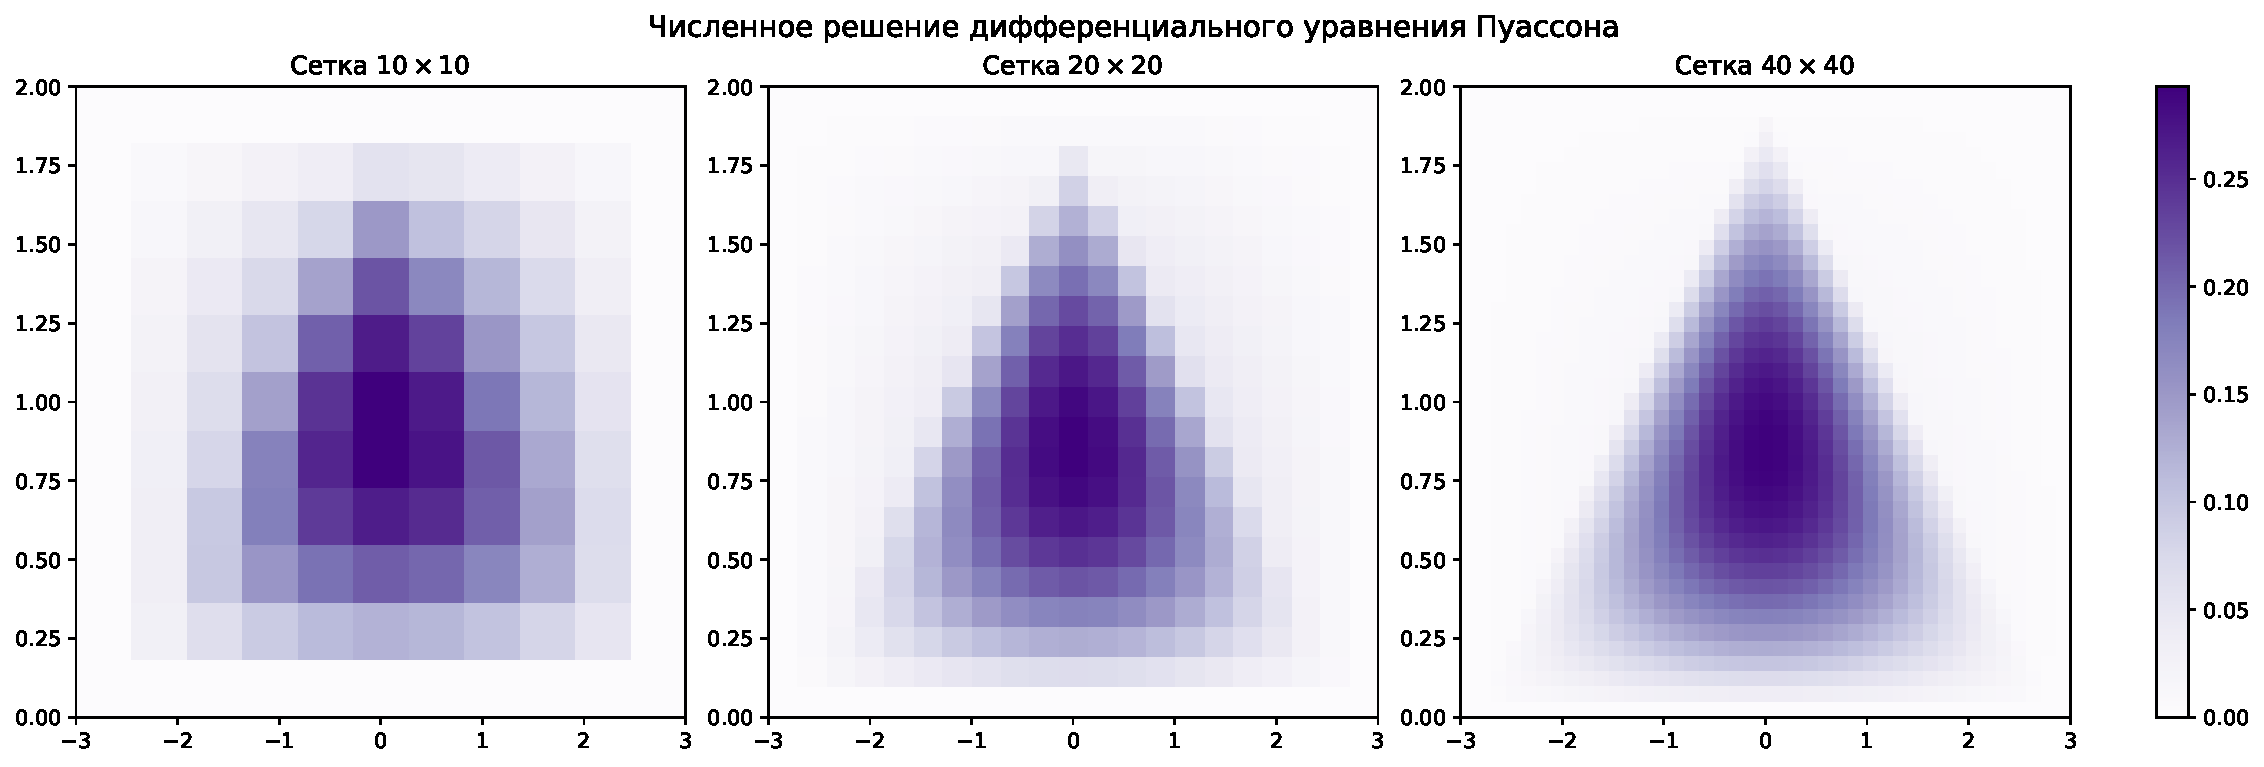
\includegraphics[width=\linewidth]{figs/heatmaps.pdf}
        \caption{Приближенное решение для сеток малых размеров.}
        \label{fig:heatmaps}
    \end{figure}
    

    \section{Применение OpenMP}

    На следующем этапе была разработана параллельная версия программы с применением технологии OpenMP. Цель --- ускорить вычисления за счёт распараллеливания расчетов на многопоточном процессоре при сохранении точности численного решения.
    
    При разработке OpenMP-программы были определены участки кода, поддающиеся эффективному распараллеливанию (в частности, вычисления элементов матрицы и вектора правой части системы уравнений, матричные и скалярные произведения).

    Расчёты были проведены на сетке $(M, N) = (40, 40)$ с различным количеством OpenMP-нитей — 1, 4 и 16. Результаты приведены в Таб. \ref{tab:open_small}.

    \begin{table}[h!]
        \centering
        \begin{tabular}{c|c|c|c|c}
            \hline
            Количество & Число точек & Число & Время & Ускорение \\
            OpenMP-нитей & сетки $ (M \times N) $ & итераций & решения &  \\ \hline
            1  & $40 \times 40$ & 126 & 0.029s & $1.00\times$ \\
            4  & $40 \times 40$ & 126 & 0.016s & $1.77\times$ \\
            16 & $40 \times 40$ & 126 & 0.015s & $1.95\times$ \\
        \end{tabular}
        \caption{Таблица с результатами расчётов на сетке малых размеров на ПВС IBM Polus (OpenMP код).}
        \label{tab:open_small}
    \end{table}
    
    Для измерения ускорения многопоточной реализации расчеты также были произведены на сетках $(M, N) = (400, 600), (800, 1200)$. Результаты приведены в Таб. \ref{tab:open_big} и визуализированы на Рис. \ref{fig:openmp_speedup}. Численное решение на сетке $(M, N) = (800, 1200)$ визуализировано на Рис. \ref{fig:poisson}.
    \begin{table}[h!]
        \centering
        \begin{tabular}{c|c|c|c|c}
            \hline
            Количество & Число точек & Число & Время & Ускорение \\
            OpenMP-нитей & сетки $ (M \times N) $ & итераций & решения &  \\ \hline
            2  & $400 \times 600$ & 1367 & 4.19s & $1.87\times$ \\
            4  & $400 \times 600$ & 1367 & 2.28s & $3.45\times$ \\
            8  & $400 \times 600$ & 1367 & 1.34s & $5.87\times$ \\
            16 & $400 \times 600$ & 1367 & 0.77s & $10.17\times$ \\ \hline
            4  & $800 \times 1200$ & 2599 & 17.31s & $3.26\times$ \\
            8  & $800 \times 1200$ & 2599 & 9.05s & $6.23\times$ \\
            16 & $800 \times 1200$ & 2599 & 7.88s & $7.15\times$ \\
            32 & $800 \times 1200$ & 2599 & 4.15s & $13.59\times$ \\
        \end{tabular}
        \caption{Таблица с результатами расчётов на ПВС IBM Polus (OpenMP код).}
        \label{tab:open_big}
    \end{table}


    \begin{figure}
        \centering
        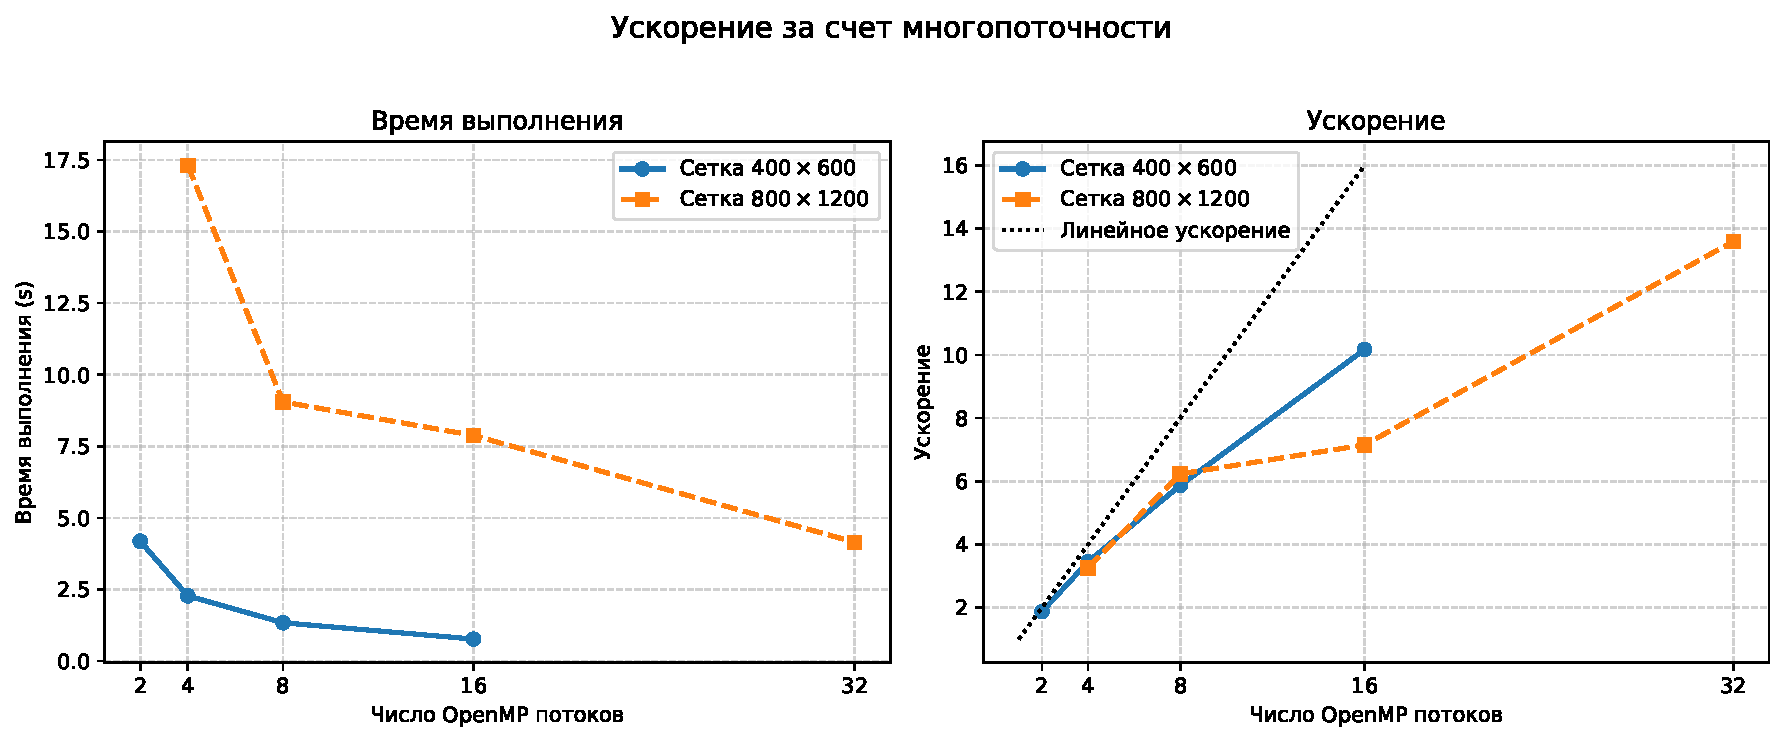
\includegraphics[width=\linewidth]{figs/openmp_speedup.pdf}
        \caption{Время работы и ускорение OpenMP программы.}
        \label{fig:openmp_speedup}
    \end{figure}

    \begin{figure}
        \centering
        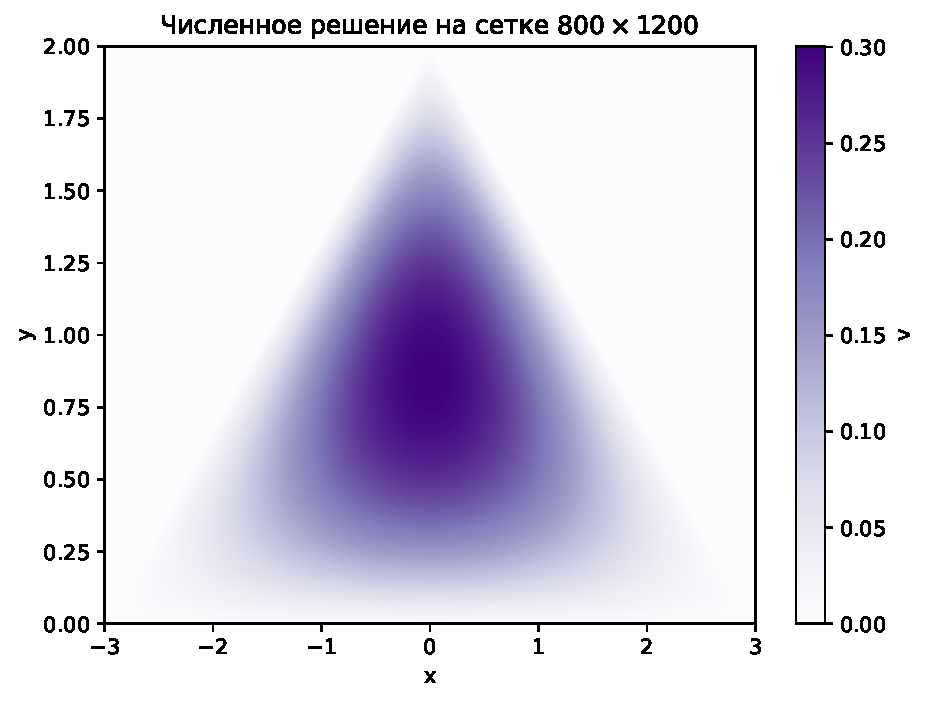
\includegraphics[width=0.65\linewidth]{figs/poisson.pdf}
        \caption{Приближенное решение уравнения Пуассона на сетке $800 \times 1200$.}
        \label{fig:poisson}
    \end{figure}


    \section{Применение MPI}

    Для реализации многопроцессной программы прямоугольная расчетная сетка была разделена на несколько прямоугольных поддоменов, каждый из которых обрабатывался отдельным MPI-процессом.

    Согласно заданию было реализовано двумерное разбиение сетки на \(p = p_x \times p_y\) поддоменов, где \(p\) — общее число запущенных MPI-процессов. Количество процессов вдоль осей \(x\) и \(y\) (\(p_x\) и \(p_y\)), выбиралось таким образом, чтобы минимизировать отклонение от единицы отношения \(p_x / p_y\) и, как следствие, обеспечить близкое к квадратному разбиение доменов. Размеры поддоменов вычислялись с учетом целочисленного деления общего числа узлов сетки на число процессов по каждому направлению, а остатки от деления равномерно распределялись между первыми процессами, что гарантирует различие в количестве узлов по каждой из осей не более чем на единицу между любыми двумя доменами.

    Каждый MPI-процесс хранит в своей памяти лишь те данные, которые относятся к его поддомену, а также данные соседних по разбиению областей, обрабатываемых другими процессами, необходимые для корректной работы пятиточечной схемы.

    Результаты расчетов, демонстрирующие эффективность MPI-реализации, представлены в Таб. \ref{tab:mpi}.

    \begin{table}[h!]
        \centering
        \begin{tabular}{c|c|c|c|c}
            \hline
            Количество & Число точек & Число & Время & Ускорение \\
            процессов MPI & сетки $ (M \times N) $ & итераций & решения &  \\ \hline
            2  & $400 \times 600$ & 1367 & 3.56s & $2.01\times$ \\
            4  & $400 \times 600$ & 1367 & 1.86s & $3.85\times$ \\
            8  & $400 \times 600$ & 1367 & 0.96s & $7.46\times$ \\
            16 & $400 \times 600$ & 1367 & 0.59s & $12.13\times$ \\ \hline
            4  & $800 \times 1200$ & 2599 & 13.39s & $4.21\times$ \\
            8  & $800 \times 1200$ & 2599 & 6.92s & $8.19\times$ \\
            16 & $800 \times 1200$ & 2599 & 3.75s & $15.15\times$ \\
            32 & $800 \times 1200$ & 2599 & 2.26s & $25.09\times$ \\
        \end{tabular}
        \caption{Таблица с результатами расчётов на ПВС IBM Polus (MPI код).}
        \label{tab:mpi}
    \end{table}


    \section{Гибридная реализация}

    В данной реализации MPI используется для организации межпроцессного взаимодействия, а технология OpenMP -- для распараллеливания вычислений внутри одного MPI-процесса с использованием доступных ему процессорных ядер.

    За основу была взята разработанная ранее MPI-программа. Декомпозиция области и межпроцессные обмены остались без изменений. Средства OpenMP были применены для распараллеливания вычислительно интенсивных циклов, которые каждый MPI-процесс выполняет над своим локальным поддоменом.

    Директивы OpenMP были добавлены в следующие участки кода:

    \begin{itemize}
        \item Циклы инициализации массивов;
        \item Векторные операции;
        \item Вычисление локальных скалярных произведений.
    \end{itemize}

    Результаты тестирования гибридной программы, показывающие эффективность совместного использования MPI и OpenMP для решения поставленной задачи, приведены в Таб.~\ref{tab:mpi_openmp}.

    \begin{table}[h!]
        \centering
        \begin{tabular}{c|c|c|c|c|c}
            \hline
            Количество & Количество & Число точек & Число & Время & Ускорение \\
            процессов & OpenMP-нитей & сетки $ (M \times N) $ & итераций & решения &  \\
            MPI & в процессе & & & &  \\ \hline
            2 & 1 & $400 \times 600$ & 1367 & 5.71s & $1.38\times$ \\
            2 & 2 & $400 \times 600$ & 1367 & 2.08s & $3.79\times$ \\
            2 & 4 & $400 \times 600$ & 1367 & 1.12s & $7.05\times$ \\
            2 & 8 & $400 \times 600$ & 1367 & 0.59s & $13.29\times$ \\ \hline
            4 & 1 & $800 \times 1200$ & 2599 & 14.83s & $4.07\times$ \\
            4 & 2 & $800 \times 1200$ & 2599 & 7.87s & $7.66\times$ \\
            4 & 4 & $800 \times 1200$ & 2599 & 4.06s & $14.87\times$ \\
            4 & 8 & $800 \times 1200$ & 2599 & 2.14s & $28.17\times$ \\

        \end{tabular}
        \caption{Таблица с результатами расчётов на ПВС IBM Polus (MPI + OpenMP код).}
        \label{tab:mpi_openmp}
    \end{table}


    \section{Реализация на CUDA}

    Для решения задачи на гибридных вычислительных системах была разработана версия программы, использующая технологию MPI для распределения памяти и вычислений между узлами, и технологию NVIDIA CUDA для ускорения вычислений внутри каждого процесса с помощью графических процессоров (GPU).

    В гибридной реализации используется стратегия декомпозиции области: расчетная сетка разбивается на прямоугольные подобласти, каждая из которых обрабатывается отдельным MPI-процессом. В начале работы программы каждый MPI-процесс выбирает соответствующее ему устройство GPU
    
    Инициализация данных происходит на хосте (CPU), после чего выполняется копирование массивов с хоста на устройство (GPU). Обратное копирование результата выполняется после удовлетворения критерия сходимости.

    Вычислительно трудоемкие операции вынесены в отдельные CUDA-ядра, среди которых:

    \begin{itemize}
        \item действие сеточного оператора на промежуточную сеточную функцию;
        \item векторные сложения, вычитания, умножения, деления;
        \item подсчеты скалярных произведений и норм.
    \end{itemize}

    Расчеты проводились на одной и двух GPU NVIDIA Tesla P100, а также без использования графических ускорителей для замера ускорений. Помимо общего времени работы программы (\(T_{total}\)), замерялось также время инициализации весов и параметров метода сопряженных градиентов (\(T_{init}\)), время работы итерационного процесса (\(T_{loop}\)), а также суммарное время коммуникаций между устройствами (\(T_{comm}\)). Результаты замеров приведены в Таб. \ref{tab:cuda}.


    \begin{table}[h!]
        \centering
        \small
        \begin{tabular}{c|c|c|c|c|c|c|c|c}
            \hline
            Количество & Количество & Число точек & Число & \(T_{total}\) & \(T_{init}\) & \(T_{loop}\) & \(T_{comm}\) & Ускорение \\
            процессов & GPU & сетки $ (M \times N) $ & итер. & (s) & (s) & (s) & (s) & цикла ($\times$) \\
            MPI & & & & & & & &  \\ \hline
            1 & - & $400 \times 600$ & 1367 & 7.64 & 0.33 & 7.31 & - & 1.00 \\
            1 & 1 & $400 \times 600$ & 1367 & 0.83 & 0.32 & 0.51 & 0.09 & 14.33 \\
            2 & 2 & $400 \times 600$ & 1367 & 0.69 & 0.19 & 0.50 & 0.10 & 14.62 \\
            \hline
            1 & - & $800 \times 1200$ & 2599 & 60.36 & 2.52 & 57.84 & - & 1.00 \\
            1 & 1 & $800 \times 1200$ & 2599 & 2.75 & 0.99 & 1.76 & 0.18 & 32.86 \\
            2 & 2 & $800 \times 1200$ & 2599 & 1.92 & 0.56 & 1.36 & 0.21 & 42.53 \\
            \hline
            1 & - & $2048 \times 2048$ & 4109 & 291.95 & 4.11 & 287.84 & - & 1.00 \\
            1 & 1 & $2048 \times 2048$ & 4109 & 12.85 & 4.53 & 8.32 & 0.37 & 34.59 \\
            2 & 2 & $2048 \times 2048$ & 4109 & 7.79 & 2.72 & 5.07 & 0.44 & 56.77 \\ \hline
            1 & - & $4096 \times 4096$ & 8020 & 3868.57 & 21.46 & 3847.11 & -   & 1.00 \\
            20 & - & $4096 \times 4096$ & 8020 & 207.87 & 1.24 & 206.63 & 0.89 & 18.62 \\
            20 $\times$ 8 & - & $4096 \times 4096$ & 8020 & 111.34 & 1.06 & 110.28 & 0.71   & 34.88 \\
            1 & 1 & $4096 \times 4096$ & 8020 & 60.22 & 19.02 & 41.20 & 0.20 & 93.38 \\
            2 & 2 & $4096 \times 4096$ & 8020 & 32.74 & 10.61 & 22.13 & 7.81 & 173.84 \\
        \end{tabular}
        \caption{Таблица с результатами расчётов на ПВС IBM Polus (MPI + CUDA код).}
        \label{tab:cuda}
    \end{table}

    Ускорение и эффективность масштабирования визуализированы на Рис. \ref{fig:cuda}. Исходя из полученных результатов, можно сделать вывод, что эффективность масштабирования растем с увеличением размеров сетки. Это ожидаемый результат, поскольку основной вклад во время работы программы вносит время итерационного процесса, в то время как время коммуникаций растет несильно.

    \begin{figure}
        \centering
        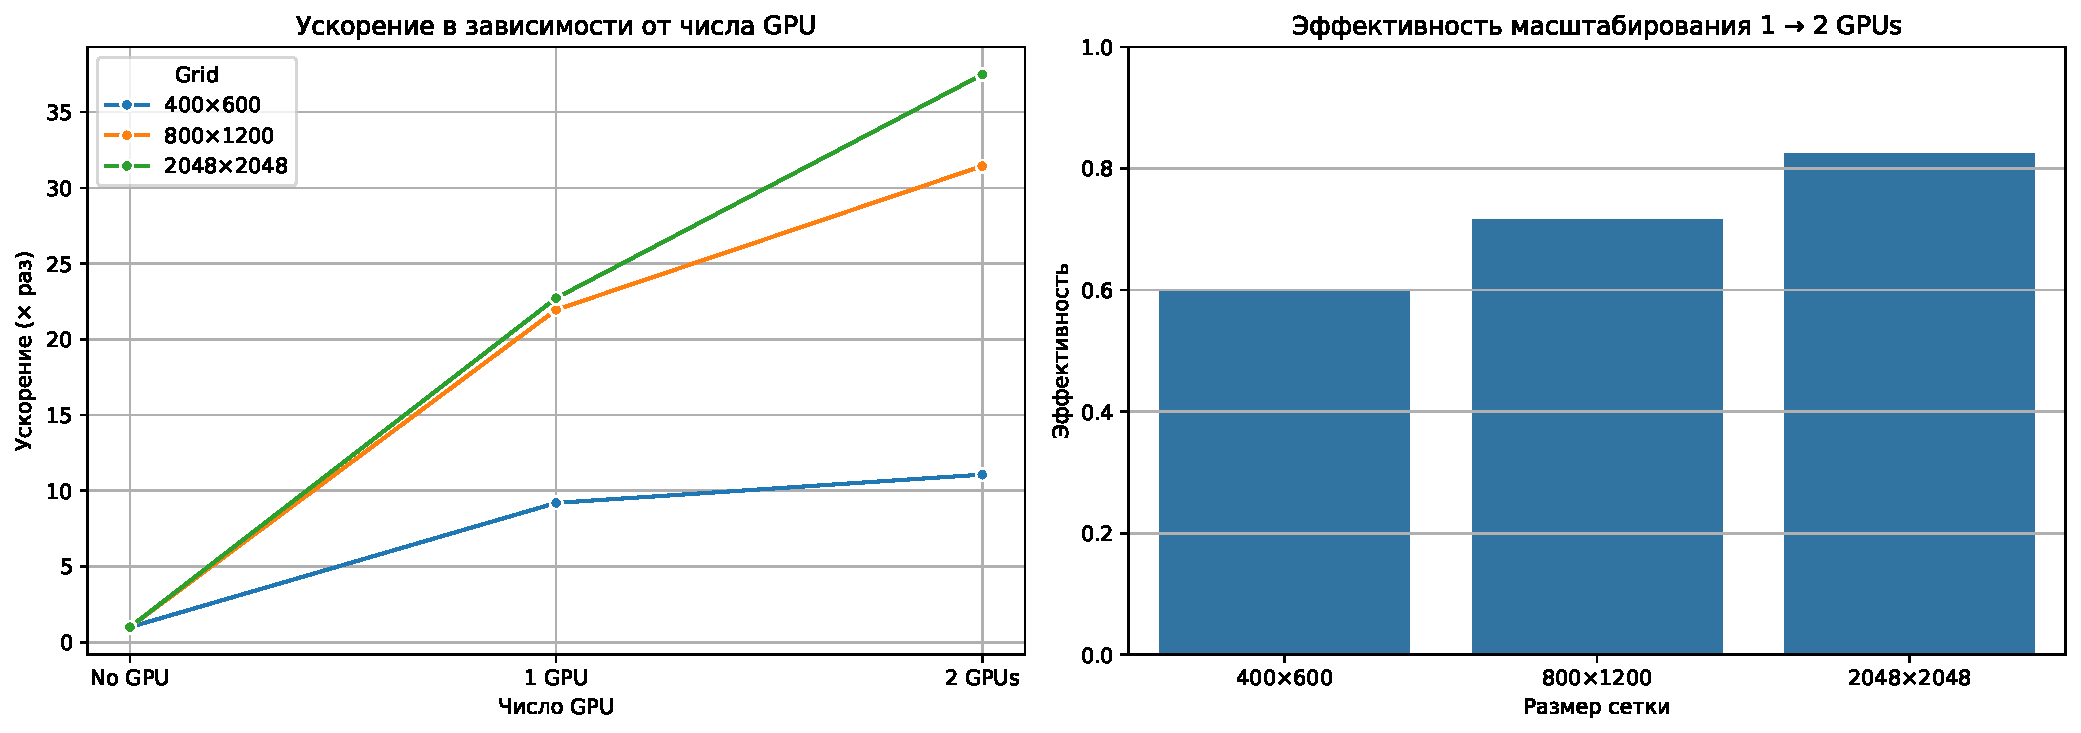
\includegraphics[width=0.95\linewidth]{figs/gpus.pdf}
        \caption{Ускорение и эффективность гибридной MPI + CUDA реализации. Ускорение приближается к линейному с ростом размера сетки.}
        \label{fig:cuda}
    \end{figure}

    
    \section{Выводы}

    В ходе работы была решена двумерная задача Дирихле для уравнения Пуассона в тупоугольном треугольнике с использованием метода фиктивных областей и метода конечных разностей. Для решения полученной системы линейных алгебраических уравнений применялся итерационный метод сопряженных градиентов.

    Были разработаны и протестированы четыре версии программы: последовательная, параллельная с использованием OpenMP, параллельная с использованием MPI и гибридная (MPI + OpenMP).
    
    На основе полученных результатов можно сделать следующие выводы:

    \begin{enumerate}
        \item Все параллельные реализации показали значительное ускорение по сравнению с последовательной версией;
        \item Реализация с использованием OpenMP продемонстрировала ожидаемое ускорение на небольшом числе потоков. Однако с ростом числа потоков до 16 и 32 ее эффективность снижалась, а ускорение замедляло свой рост (до \(\sim 13.6 \times\) на 32 потоках для сетки \(800 \times 1200\));
        \item Реализация с использованием MPI, основанная на декомпозиции области, показала значительно лучшую масштабируемость. В результате было достигнуто ускорение до \(\sim 25 \times\) на 32 процессах.
        \item Гибридная реализация (MPI + OpenMP) оказалась наиболее эффективной среди программ, не использующих графические ускорители. Комбинация MPI для межпроцессного взаимодействия и OpenMP для распараллеливания вычислений внутри каждого процесса позволила достичь наилучшего времени выполнения и максимального ускорения (\(\sim 28 \times\) на конфигурации 4 процесса по 8 потоков).
        \item Наибольшего ускорения удалось добиться при выполнений вычислений на графических ускорителях (\(\sim 173 \times\) на 2 GPU).
        \item Эффективность масштабирования по числу графических ускорителей растет с ростом сетки, который снижает вклад времени на коммуникации.
    \end{enumerate}

    Таким образом, для решения данной задачи на кластерной архитектуре ПВС IBM Polus гибридная модель является оптимальной стратегией, позволяющей добиться максимальной производительности и наилучшей масштабируемости.

\end{document}